
The characterization of \ac{URS} with the UDD condition allows us to simulate Gaussian errors and illustrate the effect of dependence on the phase transition behavior in finite dimensions.
We shall compare the performance of the Bonferroni's procedure, which is agnostic to both sparsity and signal size, with the oracle procedure which picks the top-s observations.

The first set of experiments explores short-range dependent errors from an auto-regressive (AR) models.
\begin{itemize}
	\item AR(1) Gaussian errors with parameter $\rho = -0.5$, $\rho = 0.5$, and $\rho = 0.9$,
	where the autocovariance functions decay exponentially, 
	$\rho_{k} = \rho^{k}$.
\end{itemize}
We again apply both the sparsity- and signal-size agnostic Bonferroni's procedure, i.e., $\widehat{S} = \{i:x(i)>\sqrt{2\log{p}}\}$, as well as the oracle procedure $\widehat{S}^* = \{i:x(i)\ge x_{[s]}\}$, $s=|S|$, to all settings.
Results of the numerical experiments for the AR models are shown in Figure \ref{fig:phase-simulated-dependent}.

As was commented in the main text, for dependent errors the oracle procedures is able to recover support of signals with higher probability than the Bonferroni procedures in finite dimensions; compare left and right columns of Figure \ref{fig:phase-simulated-dependent}.
Short range dependent observations, however, there is not a pronounced difference.
The results of the experiments are very similar to that of the independent Gaussian case.

\begin{figure}
    \centering
    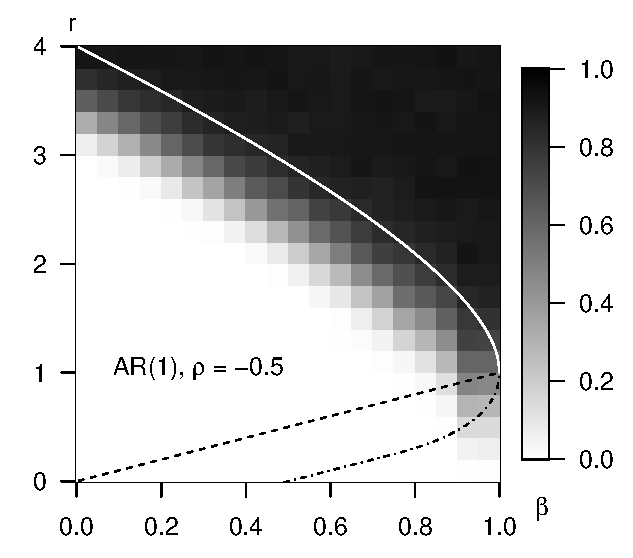
\includegraphics[width=0.4\textwidth]{./figures/simulated_phase_diagram_AR-05_p10000.eps}
    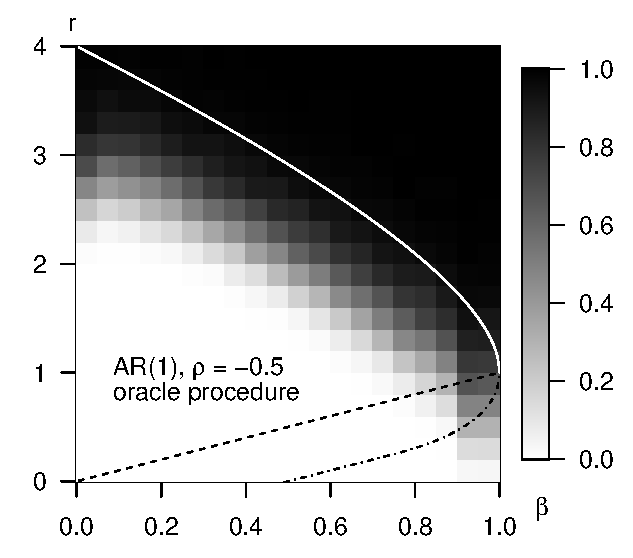
\includegraphics[width=0.4\textwidth]{./figures/simulated_phase_diagram_AR-05_p10000_oracle.eps}
    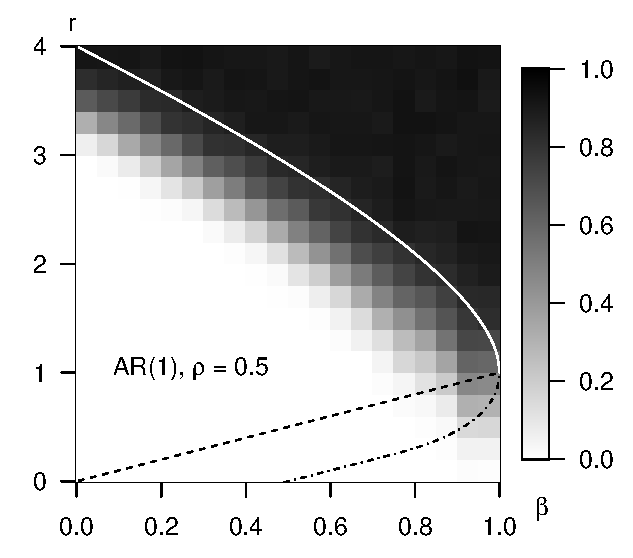
\includegraphics[width=0.4\textwidth]{./figures/simulated_phase_diagram_AR05_p10000.eps}
    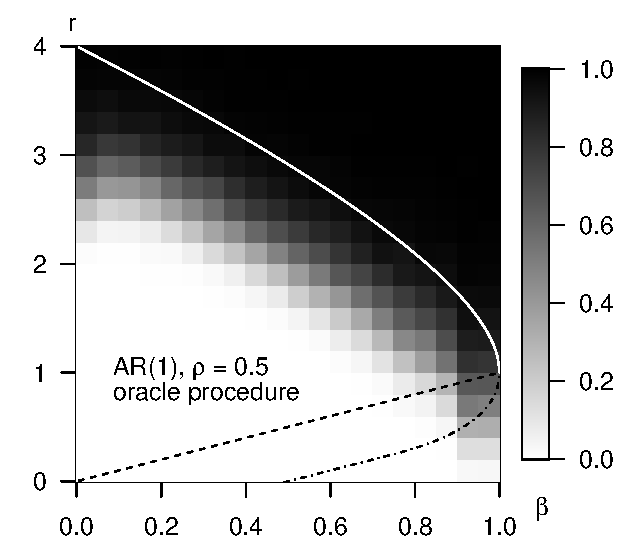
\includegraphics[width=0.4\textwidth]{./figures/simulated_phase_diagram_AR05_p10000_oracle.eps}
    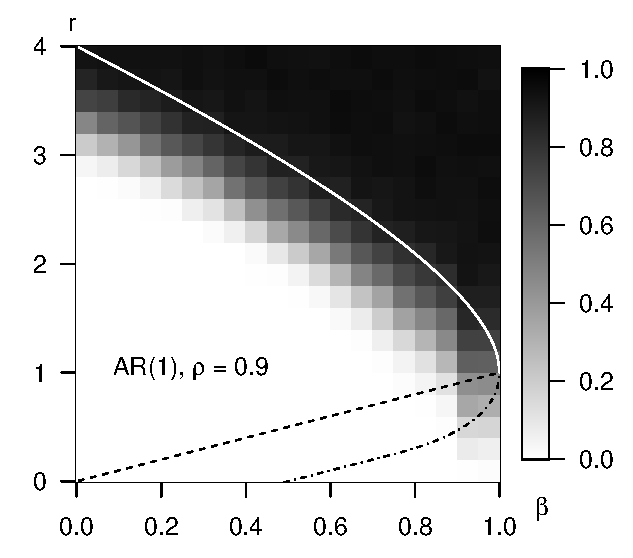
\includegraphics[width=0.4\textwidth]{./figures/simulated_phase_diagram_AR09_p10000.eps}
    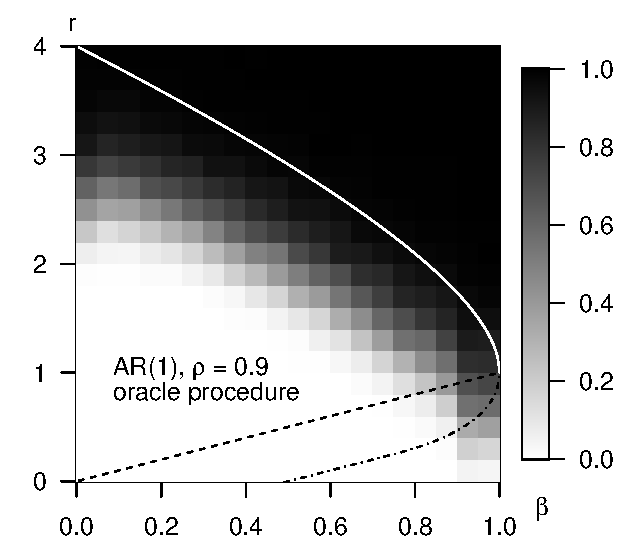
\includegraphics[width=0.4\textwidth]{./figures/simulated_phase_diagram_AR09_p10000_oracle.eps}
    \caption{The empirical probability of exact support recovery from numerical experiments, as a function of sparsity level $\beta$ and signal sizes $r$. Darker colors indicate higher probability of exact support recovery. 
    Three AR(1) models with autocorrelation functions $(-0.5)^k$ (upper), 
    $0.5^k$ (middle), and $0.9^k$ (lower) are simulated.
    The experiments were repeated 1000 times for each sparsity-signal size combination.
    In finite dimensions ($p=10000$), the Bonferroni procedures (left) suffers small loss of power compared to the oracle procedures (right).
    A phase transition in agreement with the predicted boundary \eqref{eq:strong-classification-boundary} can be seen in the AR models.
    The boundaries (solid, dashed, and dash-dotted lines) are as in Fig \ref{fig:phase-simulated}.}
    \label{fig:phase-simulated-dependent}
\end{figure}

\medskip

The second set of experiments explores exact support recovery in additive error models in the cases of long-range dependent but UDD, as well as non-UDD errors.
In particular we simulate
\begin{itemize}
    \item Fractional Gaussian noise (fGn) with Hurst parameter $H = 0.75$ and $H = 0.9$. 
    The autocovariance functions are 
    % $$\rho_{k} \sim 2H(2H-1)k^{2H-2},$$
    $$\rho_{k} \sim 0.75k^{-0.6} \quad \text{and} \quad \rho_{k} \sim 1.44k^{-0.2},$$
    as $k\to\infty$.
    Both fGn models represent the regime of long-range dependence, where covariances decay very slowly to zero, so that $\sum|\rho_k| = \infty$; see, e.g., \citep{taqqu2003livre}.
    Observe that every stationary Gaussian process with vanishing autocovariance gives rise to an UDD array as concluded in Corollary \ref{cor:stationary-Gaussian-errors}.
    \item The non-UDD Gaussian errors described in Example \ref{exmp:counter-example}.
\end{itemize}
We will apply both the sparsity-and-signal-size-agnostic Bonferroni's procedure, i.e., $\widetilde{S} = \{i:x(i)>\sqrt{2\log{p}}\}$, as well as the oracle procedure $\widehat{S}^* = \{i:x(i)\ge x_{[s]}\}$, $s=|S|$, to all settings.
Results of the numerical experiments for the fGn and non-UDD models are shown in Figure \ref{fig:phase-simulated-very-dependent}.


\begin{figure}
    \centering
    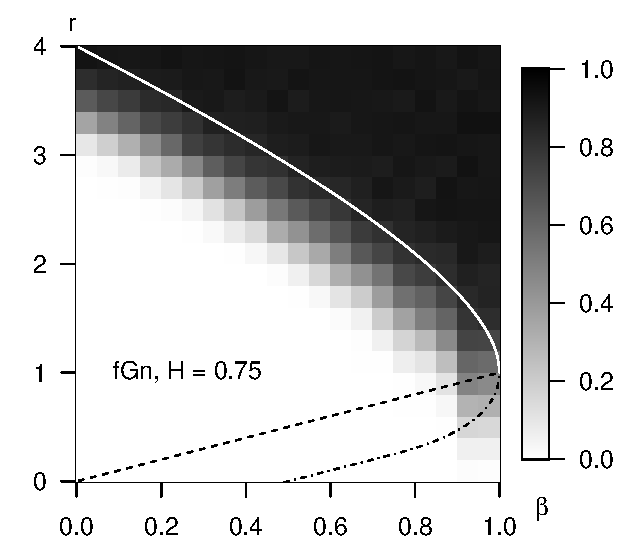
\includegraphics[width=0.4\textwidth]{./figures/simulated_phase_diagram_fGn075_p10000.eps}
    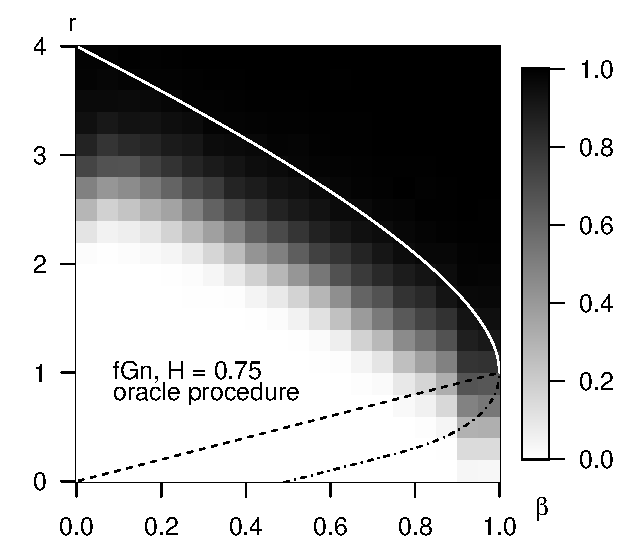
\includegraphics[width=0.4\textwidth]{./figures/simulated_phase_diagram_fGn075_p10000_oracle.eps}
    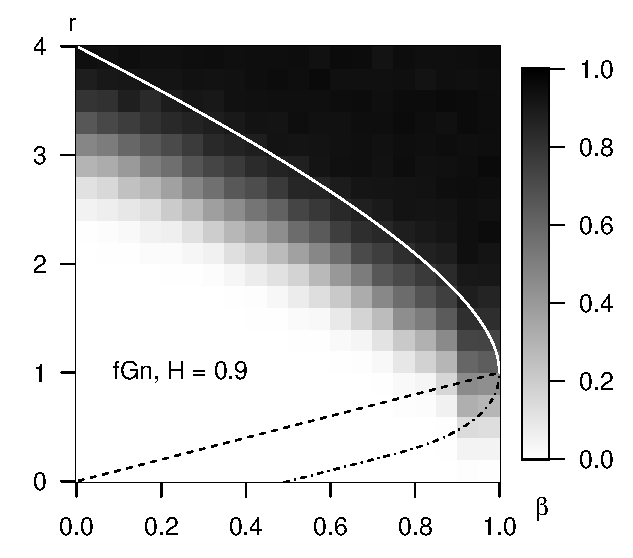
\includegraphics[width=0.4\textwidth]{./figures/simulated_phase_diagram_fGn09_p10000.eps}
    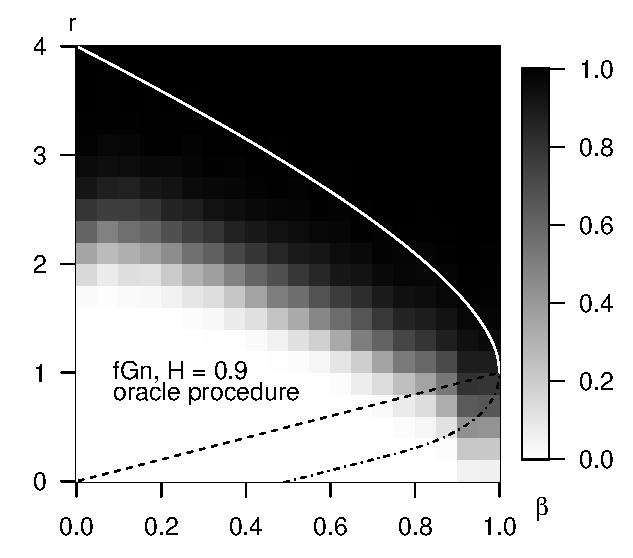
\includegraphics[width=0.4\textwidth]{./figures/simulated_phase_diagram_fGn09_p10000_oracle.eps}
    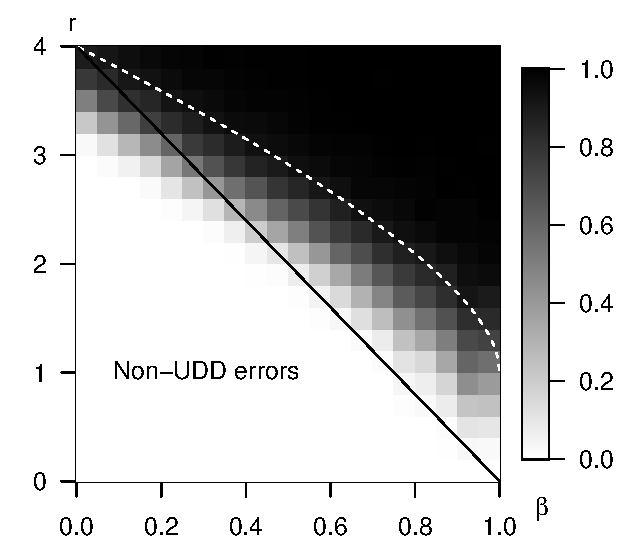
\includegraphics[width=0.4\textwidth]{./figures/simulated_phase_diagram_block_structure_p10000_agnostic7.eps}
    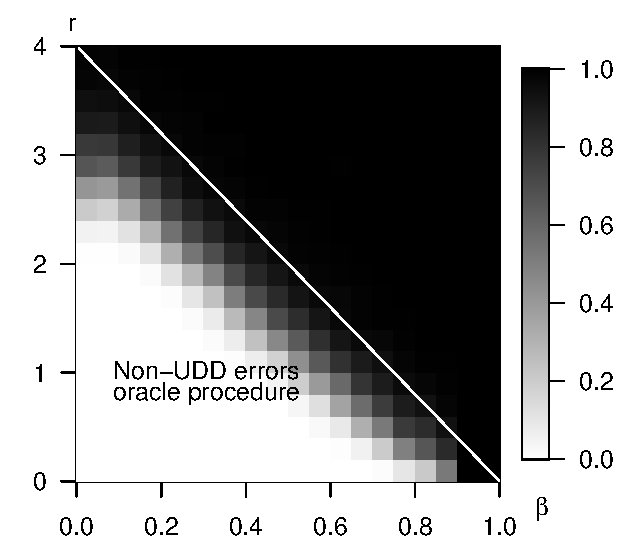
\includegraphics[width=0.4\textwidth]{./figures/simulated_phase_diagram_block_structure_p10000_oracle6.eps}
    \caption{The empirical probability of exact support recovery from numerical experiments, as a function of sparsity level $\beta$ and signal sizes $r$. Darker colors indicate higher probability of exact support recovery. 
    Two fGn models with Hurst parameter $H = 0.75$ (upper), 
    $H = 0.9$ (middle), and the non-UDD errors in Example \ref{exmp:counter-example} (lower) are simulated.
    The experiments were repeated 1000 times for each sparsity-signal size combination.
    In finite dimensions ($p=10000$), the oracle procedures (right) is able to recover support for weaker signals than the Bonferroni procedures (left) when errors are heavily dependent, although they have the same phase transition limit.
    The non-UDD errors demonstrate qualitatively different behavior, enabling support recovery for strictly weaker signals.
    The boundaries (solid, dashed, and dash-dotted lines) are as in Fig \ref{fig:phase-simulated}.
    In the non-UDD example, dashed lines represent the limit attained by Bonferroni's procedures.
    See text for additional comments.}
    \label{fig:phase-simulated-very-dependent}
\end{figure}


Notice that the oracle procedure sets its thresholds more aggressively (at roughly $\sqrt{2\log s}$) than the Bonferroni procedure (at $\sqrt{2\log p}$).
Although this difference vanishes as $p\to\infty$, in finite dimensions ($p=10\,000$) the advantage can be felt. 
Indeed, in all our experiments the oracle procedure is able to recover support of signals with higher probability than the Bonferroni procedures; compare left and right columns of Figure  \ref{fig:phase-simulated-very-dependent}.
Notice also that there is an increase in probability of recovery near $\beta=0$ for oracle procedures.
This is an artifact in finite dimensions due to the fact that $s = \lfloor p^{1-\beta}\rfloor < p/2$, and there are more signals than nulls. The oracle procedures is able to adjust to this reversal by lowering its threshold accordingly.

For UDD errors, Theorem \ref{thm:necessary} predicts that exact recovery of the support is impossible when signal sizes are below the boundary \eqref{eq:strong-classification-boundary}, even with oracle procedures. 
% Both the AR and the fGn models generate UDD Gaussian errors, and should demonstrate the same phase-transition boundary.
However, the rate of this convergence (i.e., $\P[\widehat{S}^*=S]\to0\;\text{or}\;1$) can be very slow when the errors are heavily dependent,
even though all AR and fGn models demonstrate qualitatively the same behavior in line with the predicted boundary \eqref{eq:strong-classification-boundary}. 
In finite dimensions ($p=10\,000$), as dependence in the errors increases (fGN(H=0.75) to fGN(H=0.9)), the oracle procedure becomes more powerful at recovering signal support with high probability for weaker signals. 

On the other hand, as demonstrated in Example \ref{exmp:counter-example}, non-UDD errors yield qualitatively different behavior; exact support recovery is possible for signal sizes strictly weaker than that in the UDD case. 
Lower-right panel of Figure \ref{fig:phase-simulated-very-dependent} demonstrates in this example that the signal support can be recovered as long as the signal sizes are larger than $4(1-\beta)$.

\medskip

For completeness, we verify the claims in Example \ref{exmp:counter-example}.

\begin{proof}[Proof of claims in Example \ref{exmp:counter-example}]
Recall that $\widehat{S}^* = \{j:x(j)>t_p^*\}$, where $t_p^* = \sqrt{2(1-\beta)\log{p}}$. 
Analogous to \eqref{eq:Bonferroni-FWER-control} in the proof of Theorem \ref{thm:sufficient}, we have
\begin{align*}
    \P\left[\widehat{S} \subseteq S\right] 
        &= 1 - \P\left[\max_{j\in S^c}x(j) > t_p^*\right] 
        = 1 - \P\left[\max_{j\in S^c}\epsilon(j) > t_p^*\right] \nonumber \\
      % \ge 1 - \P\left[\max_{j\in\{1,\ldots,p\}}\epsilon(j) > t_p\right] \nonumber \\
        &\ge 1 - \P\left[\max_{j\in\{1,\ldots,p\}}\epsilon(j) > t_p^*\right] 
        \ge 1 - \P\left[\max_{j\in\{1,\ldots,\lfloor p^{1-\beta}\rfloor\}}\widetilde{\epsilon}(j) > t_p^*\right]
\end{align*}
where $\left(\widetilde{\epsilon}\right)_{j=1}^{\lfloor p^{1-\beta}\rfloor}$'s are independent Gaussian errors; in the last inequality we used the assumption that there are at most $\lfloor p^{1-\beta}\rfloor$ independently distributed Gaussian errors in $\left(\epsilon_p(j)\right)_{j=1}^p$.
By Example \ref{exmp:FWER-controlling_procedures} (with $\lfloor p^{1-\beta}\rfloor$ taking the role of $p$), we know that the FWER goes to 0 at a rate of 
$\left(2\log{\lfloor p^{1-\beta}\rfloor}\right)^{-1/2}$.
Therefore, the probability of no false inclusion converges to 1.


On the other hand, since the signal sizes are no smaller than $(\nu\underline{r}\log p)^{1/\nu}$, similar to \eqref{eq:sufficient-proof-eq1}, we obtain
\begin{align}
    \P\left[\widehat{S} \supseteq S\right] 
    &\ge \P\left[\min_{j\in S}\epsilon(j) > \sqrt{2(1-\beta)\log{p})} - \sqrt{2\underline{r}\log{p}} \right] \nonumber \\
    &= \P\left[\max_{j\in S}\left(-\epsilon(j)\right) < \sqrt{2\log{p})}\left(\sqrt{\underline{r}}-\sqrt{1-\beta}\right) \right] \nonumber \\
    &= \P\left[\frac{\max_{j\in S}(-\epsilon(j))}{u_{|S|}} < \frac{\sqrt{\underline{r}}-\sqrt{1-\beta}}{\sqrt{1-\beta}}\left(1+o(1)\right) \right], \label{eq:sufficient-proof-counter-example}
\end{align}
where in the last line we used the quantiles \eqref{eq:AGG-quantiles}.
Since the minimum signal size is bounded below by $\underline{r} > 4(1-\beta)$, the right-hand-side of the inequality in \eqref{eq:sufficient-proof-counter-example} converges to a constant strictly larger than 1. While the left-hand-side, by Slepian's Lemma \cite{slepian1962one}, is stochastically smaller than a r.v. going to 1, i.e.,
\begin{equation}
  \frac{1}{u_{|S|}} \max_{j\in S}(-\epsilon(j)) \stackrel{d}{\le} \frac{1}{u_{|S|}} \max_{j\in S} \epsilon^*(j) \stackrel{\P}{\longrightarrow} 1,
\end{equation}
where $\left({\epsilon^*}\right)_{j=1}^{\lfloor p^{1-\beta}\rfloor}$'s are independent Gaussian errors.
Therefore the probability in \eqref{eq:sufficient-proof-counter-example} must also converge to 1.
\end{proof}
